\documentclass[10pt,twocolumn]{article}

% Portable working-paper format. Venue-specific style can replace this
% preamble without changing the scientific content.
\usepackage[a4paper,margin=0.72in,columnsep=0.26in]{geometry}
\usepackage[T1]{fontenc}
\usepackage[utf8]{inputenc}
\usepackage{lmodern}
\usepackage{microtype}
\usepackage{amsmath,amssymb,amsthm,mathtools}
\usepackage{booktabs,multirow,array}
\usepackage{xcolor,graphicx}
\usepackage{enumitem}
\usepackage{tikz}
\usetikzlibrary{arrows.meta,positioning,calc}
\usepackage[ruled,vlined,linesnumbered]{algorithm2e}
\usepackage[round,authoryear]{natbib}
\usepackage[colorlinks=true,citecolor=blue!45!black,
            linkcolor=blue!45!black,urlcolor=blue!45!black]{hyperref}
\setlist[itemize]{leftmargin=*,itemsep=2pt,topsep=3pt}
\setlist[enumerate]{leftmargin=*,itemsep=2pt,topsep=3pt}
\setlength{\parskip}{2pt}
\newtheorem{proposition}{Proposition}
\newtheorem{definition}{Definition}
\newcommand{\spear}{\textsc{SPEAR}}
\newcommand{\pivoi}{\textsc{PI-VOI}}
\newcommand{\E}{\mathbb{E}}
\newcommand{\R}{\mathbb{R}}
\newcommand{\D}{\mathcal{D}}
\newcommand{\M}{\mathcal{M}}
\newcommand{\A}{\mathcal{A}}
\newcommand{\cP}{\mathcal{P}}
\newcommand{\code}[1]{\texttt{#1}}

\title{\vspace{-0.5cm}\textbf{SPEAR: Learning What Evidence to Seek for\\
Parameter-Level Self-Improvement in LLM Agents}}
\author{Anonymous authors\\
\small Working manuscript; author list and affiliation to be finalized}
\date{\small October 30, 2026 \quad|\quad Conceptual draft; experiments not yet reported}

\begin{document}
\maketitle
\vspace{-0.4cm}
\begin{abstract}
Long-horizon language-model agents can recognize execution failures yet remain
poor at deciding what evidence to collect to improve their \emph{future model
parameters}. Existing reflection, retrieval, and self-adaptation techniques
address pieces of this process, but a central decision remains underspecified:
which diagnostic query is most valuable \emph{because of the parameter
intervention it enables}? We formulate this problem as parameter-intervention
value of information (\pivoi), in which the benefit of querying a teacher,
consulting documentation, or conducting a controlled probe is measured by the
expected downstream value of the best subsequently verifiable parameter update,
net of acquisition cost. We present \spear{} (Self-improvement through Probing,
Evidence Acquisition, and Reparameterization), a proposed framework coupling
a parameter-aware diagnostic policy, an evidence-conditioned functional
intervention generator, and a counterfactual acceptance-and-replay loop.
A recursive extension learns the diagnostic and intervention policies from
measured update outcomes rather than merely growing an experience archive.
We provide a falsifiable, cost-matched experimental protocol separating
incremental information from linguistic reformatting, persistent adaptation
from transient routing, and recursive improvement from memory accumulation.
\textbf{This is a method proposal: empirical claims about \spear{} are
intentionally deferred pending execution.}
\end{abstract}

\section{Introduction}
\label{sec:introduction}

An agent operating a website, software toolchain, or mobile interface can
encounter a failure in the middle of a long trajectory. A language-model
consultant may explain the error; a retrieved manual may reveal a violated
precondition; a resettable simulator may disambiguate two candidate recovery
strategies. These are fundamentally different sources of evidence.
If the goal is only to finish the \emph{current} task, the agent can use the
evidence in context and move on. If the goal is to improve \emph{future}
behavior, however, it must decide whether and how to translate the evidence
into a durable model update.

Verbal feedback and episodic memory can improve behavior without changing
model weights \citep{shinn2023reflexion}. Self-adaptation can instead produce
persistent updates: SEAL learns to generate self-edits whose resulting
fine-tuning improves performance \citep{zweiger2025seal}. Other systems jointly
modify scaffolds and weights \citep{hebbar2026sia}; parametric skill synthesis
and task-conditioned adapter prediction are increasingly capable
\citep{dery2026skillsmith,han2026kvskill,khan2026distributional}.
Consequently, asking a teacher, generating an adapter, and testing it is not
by itself a distinctive technical contribution.

We study a more specific decision. Consider two failures with deliberately
indistinguishable visible traces. In one case, the tool's schema has silently
changed; in the other, a task invariant makes the apparently valid call
incorrect. Retrieving documentation may resolve the first cause, whereas an
expert explanation or controlled counterfactual trial may be necessary for
the second. A useful learner should select evidence \emph{based on which
permanent parameter change that evidence will make possible}, not simply
which source seems relevant or reduces linguistic uncertainty.

This distinction motivates \emph{parameter-aware evidence acquisition}.
The evidence is valued through the posterior expected utility of a candidate
parameter intervention on \emph{fresh, independent trajectories}, including
training expense and retention of existing abilities. The zero-update
option is explicit. A diagnostic can thus be correct and still not be worth
acquiring if it does not change the intervention decision. Conversely, a
brief probe may be worth more than a long explanation if it reverses the
preferred parameter update.

We propose \spear{} as a research framework organized around three
interlocking objects:
\begin{enumerate}
\item \textbf{Parameter-intervention value of information (\pivoi).}
      Evaluate a source by expected improvement in the \emph{best downstream
      parameter decision}, not by source confidence or textual quality.
\item \textbf{Evidence-conditioned functional interventions.}
      Map a failure state and the gathered evidence to a constrained update
      in a reusable functional basis with a small residual, scored against
      observed intervention outcomes.
\item \textbf{Outcome-driven recursive learning.}
      Use paired candidate trials and old-skill audits to update both the
      evidence policy and the intervention generator, while separately
      verifying persistent changes to the execution model.
\end{enumerate}

The intended contribution is a \emph{testable coupling} between evidence
acquisition and parameter modification. We do not claim that value-of-information
planning, hypernetworks, functional subspaces, or recursive adaptation are
individually new. In particular, our experimental design includes strong
uncombined and fully cost-matched controls. The core falsification question is
whether a learned parameter-aware policy outperforms simple error-condition
rules and fixed evidence under matched opportunities to update.

\paragraph{Scope and status.}
This draft specifies a method and an evaluation plan, not a completed system
or a report of results. The first implementation target is a small
tool-using language model and resettable, state-checkable environments;
cross-architecture generalization and unbounded autonomous improvement are
out of scope.

\section{Related Work and Novelty Boundary}
\label{sec:related}

\paragraph{Reflection, tool use, and non-parametric experience.}
ReAct interleaves reasoning and environment actions
\citep{yao2023react}; Reflexion turns feedback into verbal memory without
weight updates \citep{shinn2023reflexion}. SkillCommit evolves reusable
external skills with behavioral validation \citep{he2026skillcommit},
and SkillEvoReg controls overfitting and regressions in such evolving
skill libraries \citep{nie2026skillevoreg}. These systems motivate
credible baselines: the ability to act on feedback is not sufficient
evidence for enduring parametric learning.

\paragraph{Self-editing and text-to-parameters.}
SEAL directly trains a model to emit effective self-edit instructions
\citep{zweiger2025seal}, making it an especially close reference for
recursive parameter adaptation. SIA jointly optimizes agent scaffolds and
weights \citep{hebbar2026sia}. SkillSmith composes textual knowledge and
parameterized prefix skills \citep{dery2026skillsmith}; KV-Skill learns
loadable operators from text or rewards \citep{han2026kvskill}.
Query-conditioned distributional hypernetworks generate distributions
over LoRA updates \citep{khan2026distributional}. W2T predicts attributes
from canonicalized LoRA weights \citep{han2026w2t}; BQ-LoRA models
functional equivalence of agent updates \citep{zhou2026bqlora}.
None of these observations licenses a claim that text-to-weight
generation or functional weight geometry originated here.
\spear{} instead asks how an agent should \emph{acquire evidence} to
select and validate a durable update, conditional on the actual
post-update benefit.

\paragraph{Value of information, adaptive resources, and optimization.}
Decision-theoretic information acquisition predates language agents.
Recent work uses value of information for agent clarification
\citep{dong2026voi} and for budgeted activation of LoRA experts
\citep{saliencro2026vimole}. DeepControl studies adaptive evidence
retrieval for \emph{inference-time reasoning}
\citep{xiong2026deepcontrol}. Low-dimensional optimization of
meaningful adaptation directions also has precedents in Hyper-ES
\citep{gu2026hyperes} and CoPES \citep{wang2026copes}.
Our proposed distinction is an \emph{intervention-conditioned acquisition
objective}: a document, critique, or experiment is useful only insofar as
it changes a future model-modification decision that survives validation.

\paragraph{Parameter-efficient learning and continual retention.}
LoRA provides practical low-rank parameter interventions
\citep{hu2021lora}. Catastrophic forgetting motivates old-task audits
and guarded acceptance rules \citep{kirkpatrick2017overcoming}.
We treat preservation of previous capabilities as a measured objective,
not an assumed property of restricting update rank.

\paragraph{Closest-counterpart summary.}
SEAL optimizes self-edit outcomes but does not, in its stated formulation,
study \emph{which heterogeneous diagnostic evidence source to acquire}
according to its value for the next parameter decision. SkillSmith and
KV-Skill operationalize knowledge-to-parameter mappings but do not
directly establish parameter-aware active diagnostic source selection.
VOI-based clarification/retrieval methods optimize decisions over answers
or computation rather than validated long-term parameter changes.
These are \emph{hypothesized} distinctions to test, not a claim that
the literature has been exhaustively searched or that a combination
necessarily provides a publishable advance.

\section{SPEAR: Parameter-Aware Self-Improvement}
\label{sec:method}

\begin{figure*}[t]
\centering
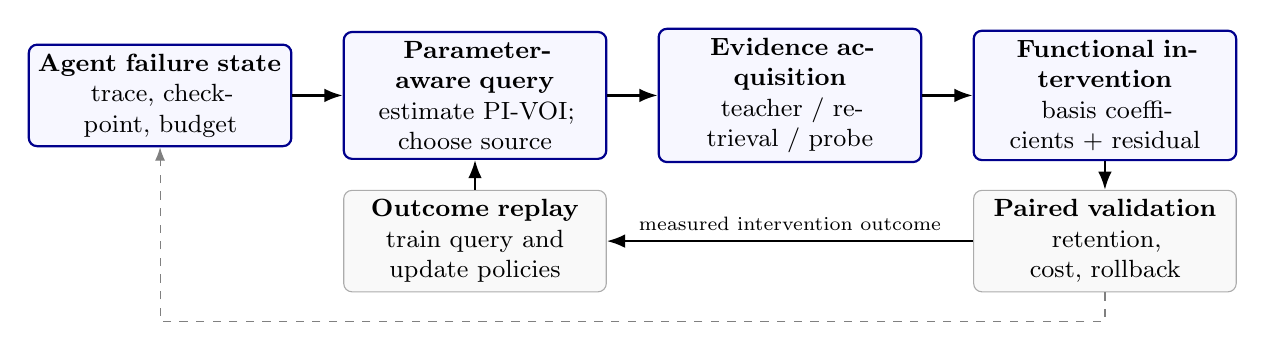
\begin{tikzpicture}[>=Latex, every node/.style={font=\small},
  stage/.style={draw=blue!55!black,rounded corners=3pt,thick,
  fill=blue!3,align=center,minimum height=0.95cm,text width=3.1cm},
  minor/.style={draw=gray!65,rounded corners=3pt,
  fill=gray!5,align=center,minimum height=0.85cm,text width=3.1cm}]
\node[stage] (failure) at (1.7,0) {\textbf{Agent failure state}\\trace, checkpoint, budget};
\node[stage] (query) at (5.7,0) {\textbf{Parameter-aware query}\\estimate PI-VOI; choose source};
\node[stage] (evidence) at (9.7,0) {\textbf{Evidence acquisition}\\teacher / retrieval / probe};
\node[stage] (propose) at (13.7,0) {\textbf{Functional intervention}\\basis coefficients + residual};
\node[minor] (verify) at (13.7,-1.85) {\textbf{Paired validation}\\retention, cost, rollback};
\node[minor] (replay) at (5.7,-1.85) {\textbf{Outcome replay}\\train query and update policies};
\draw[->,thick] (failure.east)--(query.west);
\draw[->,thick] (query.east)--(evidence.west);
\draw[->,thick] (evidence.east)--(propose.west);
\draw[->,thick] (propose.south)--(verify.north);
\draw[->,thick] (verify.west)--node[above,font=\scriptsize]{measured intervention outcome}(replay.east);
\draw[->,thick] (replay.north)--(query.south);
\draw[->,dashed,gray] (verify.south) -- ++(0,-0.37) -| (failure.south);
\end{tikzpicture}
\caption{Proposed \spear{} loop. The diagnostic policy is trained on
\emph{verified post-update outcomes}, not the superficial correctness of
an explanation. A candidate can be rejected or replaced by a no-update
decision; only an accepted update persists to future episodes.}
\label{fig:architecture}
\end{figure*}

\subsection{Decision State and the Update Objective}
Let $\theta_t\in\R^d$ denote the \emph{persistent} parameters of a
student agent at improvement round $t$. A long-horizon interaction
produces a partial trajectory $h_t=(o_0,a_0,\ldots,o_k)$ that contains
an observed failure or capability gap. The decision state is
\begin{equation}
s_t=(h_t,\theta_t,D_t,b_t,\M_t),
\end{equation}
where $D_t$ is a functional update basis, $b_t$ is the remaining
resource budget, and $\M_t$ is a log of prior evidence decisions,
parameter proposals, and evaluated outcomes. A source action
$a\in\A_{\mathrm{src}}$ may query a teacher, retrieve external
documentation, run a controlled environment probe, or stop.
An outcome $e\sim P_t(e\mid s_t,a)$ includes the acquired content,
source, cost, timestamp, and provenance. The distribution $P_t$ is
unknown and may vary with model checkpoint and environment version.

The available parameter interventions constitute a bounded set
$\Delta_t$, augmented with $\delta=0$; the latter is important because
the correct decision can be to retain the current checkpoint.
A \emph{memory-only} remedy is a separate non-parametric comparator:
it may improve current-task utility but does not count as durable
parameter improvement.

Let $\mathcal{T}^{\rm new}_t$ be independent future task instances from
the target skill distribution and $\mathcal{T}^{\rm old}_t$ a retention
suite of previously learned tasks. Denote strict episode success by
$S(\theta;z)\in[0,1]$, evaluated by the environment's state checker.
Define the net \emph{update value}
\begin{align}
J_t(\delta) ={}&
  \E_{z\sim\mathcal{T}^{\rm new}_t}[S(\theta_t+\delta;z)]
     \nonumber\\
 &-\lambda_F\Big[
     \E_{z\sim\mathcal{T}^{\rm old}_t}
     \big(S(\theta_t;z)-S(\theta_t+\delta;z)\big)
   \Big]_+ \nonumber\\
 &-\lambda_U C_{\rm update}(\delta).
\label{eq:updatevalue}
\end{align}
Here $[x]_+=\max(x,0)$ and $C_{\rm update}$ accounts for actual
training, evaluation, and deployment cost; the separate source cost is
denoted $c_{\rm src}(a)$. The weights and normalization must be fixed
\emph{before} testing. Performance on a final held-out test set must
not enter training, policy selection, or the acceptance gate.

\subsection{Parameter-Intervention Value of Information}
\label{sec:pivoi}
Given history $\M_t$, define the conditional expected utility of
an intervention after observing possible evidence $e$:
\begin{equation}
\mu_t(\delta\mid s_t,e,\M_t)
=\E[J_t(\delta)\mid s_t,e,\M_t].
\label{eq:mu}
\end{equation}
The proposed one-step \emph{parameter-intervention value of
information} for a source action is
\begin{align}
V^{\rm PI}_t(a\mid s_t,\M_t)
={}&\E_{e\sim P_t(\cdot\mid s_t,a)}
  \left[
  \max_{\delta\in\Delta_t\cup\{0\}}
  \mu_t(\delta\mid s_t,e,\M_t)
  \right]\nonumber\\
 &-\max_{\delta\in\Delta_t\cup\{0\}}
  \mu_t(\delta\mid s_t,\M_t)
  -c_{\rm src}(a).
\label{eq:pivoi}
\end{align}
The second term is the best available parameter decision without
paying for further evidence. Crucially, a source is not rewarded
for reducing uncertainty unless the reduction improves the
\emph{downstream intervention choice}. This is a decision-dependent
instance of classical value of information, \emph{not} a new
information-theoretic identity.

\begin{proposition}[Nonnegative gross value under ideal decisions]
\label{prop:voi}
Suppose the source does not itself alter $\theta_t$, all candidate
interventions remain available, the utility model is Bayes-correct,
and source cost is zero. Then the first two terms of
Eq.~\eqref{eq:pivoi} have nonnegative difference.
\end{proposition}
\noindent\textit{Proof.}
Let $\delta^\star$ maximize expected utility before acquisition.
After seeing $e$, the decision-maker can always select
$\delta^\star$. Taking expectations over $e$ and applying the law
of iterated expectations yields an expected post-query optimum
no smaller than the pre-query optimum. \hfill$\square$

This result is only an ideal benchmark: when queries are costly,
evidence is distribution-shifting, or $\mu_t$ is miscalibrated,
the estimated net value and the \emph{realized} gain can be negative.
A myopic policy chooses
$a_t=\arg\max_a\widehat V^{\rm PI}_t(a\mid s_t,\M_t)$
when that maximum is positive, otherwise stopping.
Sequential acquisition re-evaluates the same criterion after each
observation within budget. A one-step approximation does not
generally solve the optimal multi-step experimental-design problem.

\subsection{Estimating Parameter-Aware Evidence Value}
\label{sec:valuelearning}
We propose a learned intervention-value model
$Q_\omega(s,e,\delta)$, trained to predict the measured change
$J_t(\delta)-J_t(0)$, together with a calibrated uncertainty estimate
$\sigma_\omega$. For each randomized evidence decision and feasible
candidate $\delta$, the training log stores the \emph{actual} paired
validation outcome, cost, environment seed, and versioned checkpoint.
The conditional evidence model
$\widehat P_\xi(e\mid s,a)$ is optional; a direct
source-value regressor is a lower-complexity alternative when sampling
full textual evidence is impractical.

A practical source-value estimator simulates a limited set of
candidate evidence outcomes and updates:
\begin{equation}
\widehat V^{\rm PI}(a)
= \frac{1}{K}\sum_{i=1}^K
 \max_{\delta\in\widehat\Delta(s,e_i)}
 Q_\omega(s,e_i,\delta)
 -\max_{\delta\in\widehat\Delta(s)}
 Q_\omega(s,\varnothing,\delta)-c_{\rm src}(a).
\label{eq:est}
\end{equation}
Here $e_i\sim\widehat P_\xi(\cdot\mid s,a)$ and every candidate set
includes zero. This is an \emph{approximation}, not an unbiased
counterfactual estimator. Limited candidate search and maximization
of noisy scores can be optimistic; calibration on a separate
validation split, uncertainty penalties, and occasional random
source exploration are necessary. Logged source propensities must
be retained for subsequent off-policy evaluation.

\subsection{Evidence-to-Functional Intervention}
\label{sec:generator}
Let $D_t\in\R^{d\times k}$ comprise $k\ll d$ reusable parameter
directions from previously \emph{validated} updates. The proposed
generator predicts both basis coefficients and a bounded residual:
\begin{equation}
\delta_\phi(s_t,e)=
    D_t g_\phi(s_t,e)+r_\phi(s_t,e),\qquad
    \|r_\phi\|_2\le \kappa,\ \|\delta_\phi\|_2\le R.
\label{eq:functional}
\end{equation}
For large weight matrices, $r_\phi$ can be represented by small
low-rank factors or omitted in the minimal implementation.
The generator receives structured history and evidence provenance,
not just the consultant's natural-language answer. A finite library
of pre-trained directions with learned mixture coefficients is a
crucial low-cost baseline for the full generator.

A value-grounded training objective is
\begin{align}
\mathcal{L}_{\rm int}(\phi)
={}&-\E_{(s,e)\sim\M}
 \big[Q_\omega(s,e,\delta_\phi(s,e))\big]\nonumber\\
 &+\lambda_{\rm res}\|r_\phi(s,e)\|_2^2
 +\lambda_{\rm trust}\|\delta_\phi(s,e)\|_2^2.
\label{eq:generatorloss}
\end{align}
The model must not trust this surrogate alone; it proposes candidates
for \emph{real execution}, and a high predicted value is not a
validation pass. Direction reuse can be expanded only after
independently verified improvements. Directions must be attached
to a compatible checkpoint, layer layout, and parameter
normalization; cross-backbone transfer is not assumed.

\subsection{Counterfactual Acceptance and Persistence}
\label{sec:verification}
Each candidate update is evaluated against the \emph{same}
pre-update checkpoint on paired, independently initialized task
instances. For every evaluation seed, run both $\theta_t$ and
$\theta_t+\delta$ from equivalent environment state, recording
strict success and side effects. Keep data used to create the
candidate disjoint from its validation data, and never select on
the final test split. An acceptance rule can require a positive
pre-specified lower confidence bound on the new-skill gain and an
old-skill regression below tolerance $\epsilon_F$:
\begin{equation}
\mathrm{LCB}_{1-\alpha}(\Delta U_{\rm new})>0,\quad
\mathrm{UCB}_{1-\alpha}(F_{\rm old})\le\epsilon_F.
\label{eq:accept}
\end{equation}
The confidence construction, multiplicity correction, and number
of repeats must be pre-registered. When either check fails,
rollback to $\theta_t$; accept $\delta=0$ if no proposal passes.

When accepted, \emph{persist} the update as a versioned adapter or
merge it into a new checkpoint, yielding
$\theta_{t+1}=\theta_t+\delta_t^\star$.
At the next evaluation episode, disable the original teacher
message and retrieved document. If improvements require reloading
temporary query-specific adapters or re-injecting the diagnosis,
classify the effect as transient adaptation rather than persistent
parameter learning.

\subsection{Recursive Learning of the Update Mechanism}
\label{sec:recursive}
Define the learned self-improvement machinery as
$\psi_t=(\eta_t,\phi_t,\omega_t,\xi_t)$, where $\eta_t$
is the diagnostic source policy, $\phi_t$ the generator, and the
remaining components are value/evidence predictors.
After each verified trial, update
\begin{equation}
(\theta_t,\psi_t,\M_t)
\longrightarrow
(\theta_{t+1},\psi_{t+1},\M_{t+1}).
\label{eq:recursion}
\end{equation}
A constrained contextual-bandit or off-policy policy-gradient
loss for $\eta$ can use \emph{measured intervention gain minus
acquisition cost}, with recorded randomized action propensities.
The generator is trained with Eq.~\eqref{eq:generatorloss} and
ground-truth acceptance/rejection feedback. All outcomes are
versioned because $Q_\omega$ at a prior $\theta_t$ need not
generalize to the next checkpoint.

\begin{algorithm}[t]
\caption{Proposed SPEAR improvement round (research protocol)}
\label{alg:spear}
\DontPrintSemicolon
\KwIn{checkpoint $\theta_t$, failure history $h_t$, budget $b_t$,
      replay $\M_t$, candidate set $\Delta_t\cup\{0\}$}
initialize $e\leftarrow\varnothing$; source log $L\leftarrow\varnothing$\;
\While{budget remains}{
  estimate source values $\widehat V^{\rm PI}(a\mid s_t,e,\M_t)$\;
  \If{$\max_a\widehat V^{\rm PI}(a)\le 0$}{break}
  choose source $a$ (with logged exploration propensity)\;
  acquire evidence $e_a$; append $(a,e_a,c_a)$ to $L$\;
  update evidence context $e\leftarrow e\cup\{e_a\}$\;
}
generate bounded candidate updates from $(s_t,e)$, including $0$\;
evaluate candidates and unchanged checkpoint on paired validation\;
accept guarded best candidate or rollback to $\theta_t$\;
log source actions, all candidate outcomes, and retention checks\;
update $\eta,\phi,\omega$ from intervention-outcome replay\;
\KwOut{persistent $\theta_{t+1}$, updated mechanism, versioned $\M_{t+1}$}
\end{algorithm}

A claim of \emph{recursive self-improvement} must be based on an
\emph{incremental effect of learning $\psi$}. Growth of $\M_t$ alone
is not sufficient: a frozen source policy and frozen generator
must be compared with the adaptive versions under \emph{the same}
memory content, number of candidate evaluations, and task stream.
Only a reliable positive meta-learning effect supports the
recursive part of the claim.

\subsection{Distinguishing Information Gain From Rephrasing}
If a teacher diagnosis is a deterministic function of the entire
observed trace, it adds no Shannon information about a latent
environment state conditional on that trace. It can nonetheless
provide a computational advantage to a bounded-capacity generator
by making the relevant pattern easier to use. The evaluation
therefore separates (i) \emph{new external observations} from
(ii) \emph{trace-only linguistic transformations}, and does not
conflate either with successful weight-space learning.

\section{Experimental Design: Pre-registered, Not Yet Run}
\label{sec:experiments}
We organize evaluation around \emph{falsification}, not around maximizing
a single benchmark score. No numerical outcomes for \spear{} are available
in this manuscript. The protocol and a fuller execution checklist are
provided in \code{EXPERIMENTS.md}.

\subsection{Research Questions and Testbeds}
\textbf{RQ1: Is external evidence causally useful for parameter updates?}
Can acquiring evidence improve the \emph{validated future-task utility}
of a parameter intervention over a trace-only update at matched cost?

\textbf{RQ2: Does parameter-aware source selection matter?}
When two failures have the same observable surface state, can a learned
policy select different evidence sources for different latent causes
and outperform fixed sources, confidence, and hand-written rules?

\textbf{RQ3: Is the improvement persistent and retention-aware?}
Does a committed update improve full trajectories on new task
instances with all auxiliary evidence disabled, without unacceptable
regression on previously learned skills?

\textbf{RQ4: Does the improvement process itself improve?}
With identical experience-log growth, does continuing to train
the query and intervention policies improve the cost to learn
\emph{later} skills compared with frozen meta-components?

\paragraph{Stage A: controlled diagnosis environment.}
Construct a resettable tool-use simulator with failures caused by
hidden schema changes, task-invariant violations, or environment-state
preconditions. Hold the visible error string and pre-query history
constant across selected pairs. Equip each source with distinct,
controlled access (manual snippet, advisory explanation, or executable
probe); test whether evidence changes the \emph{optimal update}
rather than merely identifying a label. Generate held-out
combinations of names, tool schemas, causal mechanisms, and
trajectory lengths. Randomize source availability/order to avoid
position shortcuts. A nontrivial subset must contain a
\emph{counterfactual reversal}: within the same visible failure
condition, the best validated update differs across hidden causes.

\paragraph{Stage B: interactive agent environments.}
Evaluate transfer to AppWorld \citep{trivedi2024appworld}, which
provides state-based unit tests for interactive tool use, and
AndroidWorld \citep{rawles2024androidworld}, which provides
parameterized mobile tasks and state-based checkers. Begin with
a compact instruction-tuned student (candidate:
Qwen3.5-4B, subject to reproducibility checks). Inject only
documented, reproducible capability gaps; distinguish benchmark
limitations (for example, failed resets or unavailable tool effects)
from agent failures. Use full-trajectory strict checker success,
not a language-model judgment, as the primary endpoint.
No outcomes from Stage A should be copied into a Stage B result.

\paragraph{Evaluation splits.}
Separate (i) intervention-proposal training, (ii) within-round
candidate-selection validation, (iii) meta-policy development,
and (iv) final untouched testing, at the \emph{mechanism/skill}
and task-instance levels. Keep old-skill retention suites fixed.
For sequential learning, reveal skill families in stages; later
test instances are unavailable during earlier adaptation.
Snapshot environments and version all evidence.

\subsection{Cost-Matched Comparators}
\label{sec:baselines}
\begin{table*}[t]
\centering
\small
\setlength{\tabcolsep}{5pt}
\begin{tabular}{p{3.3cm}p{4.2cm}p{4.0cm}p{4.2cm}}
\toprule
\textbf{Method} & \textbf{Evidence acquisition} &
\textbf{Parameter update} & \textbf{Isolated comparison}\\
\midrule
Unchanged student / memory-only &
None or experience retrieval &
None & Need for parameter change vs.\ external memory\\
Fixed Teacher + SFT &
Teacher on every eligible failure &
Gradient-based supervised update &
Standard verbal feedback and fine-tuning\\
Fixed Sources + Hypernetwork &
Fixed source order/bundle &
Evidence-conditioned adapter predictor &
Parameter generator without active evidence choice\\
Contextual BO / functional ES &
Budgeted trials selected from historical gain &
Low-dimensional update search &
Generic black-box optimization of updates\\
Heuristic / confidence routing &
Simple error rules or confidence thresholds &
Same update generator as full method &
Whether learned \pivoi{} beats trivial routing\\
Evidence Policy Only &
Learned source policy &
Frozen update generator &
Marginal benefit of acquisition learning\\
Intervention Model Only &
Fixed source policy &
Learned functional intervention generator &
Marginal benefit of intervention learning\\
Full \spear{} &
Learned parameter-aware source policy &
Learned functional generator; guarded updates &
Effect of joint decision coupling\\
Frozen-meta \spear{} &
Frozen policies; replay archive still grows &
Frozen generator; matched archive and budget &
Gain attributable to recursive learning\\
\bottomrule
\end{tabular}
\caption{Planned controls. All methods should receive a comparable
source-query, candidate-evaluation, and GPU-hour budget, and
the same versioned task stream. Results are intentionally absent.}
\label{tab:baselines}
\end{table*}

The most important comparisons are \emph{not} with the weakest
student: the main claim must survive (a) simple deterministic
routing, (b) fixed expert evidence, (c) a standard update mechanism
with an adaptive source selector, and (d) a strong learned update
mechanism with fixed sources. Where a named baseline has
unavailable code, describe and validate the faithful
reimplementation instead of claiming an exact reproduction.

\subsection{Metrics and Estimands}
\label{sec:metrics}
\begin{itemize}
\item \textbf{Primary endpoint:} strict end-to-end success on
      independent \emph{new} task instances after an accepted
      parameter update, at matched cumulative budget.
\item \textbf{Sample and cost efficiency:} verified skill gain per
      teacher call, retrieval call, simulator probe, GPU-hour,
      trained token, and total normalized expense.
\item \textbf{Retention:} average drop and worst-skill drop on the
      pre-registered old-task suite, with side-effect violations.
\item \textbf{Value prediction:} signed prediction error, ranking
      regret, calibration, and false-acceptance rate of
      $Q_\omega$ and estimated \pivoi{}.
\item \textbf{Source-policy increment:} paired utility relative to
      fixed sources, confidence, and best hand-written rule
      under matched queries and candidate counts.
\item \textbf{Recursive gain:} area under the skill-acquisition
      curve, later-skill improvement per expense, and adaptive
      minus frozen-meta learning efficiency at identical replay size.
\end{itemize}

The primary causal estimand is the \emph{difference in post-update
utility under a randomized evidence-source policy} at a fixed
checkpoint and intervention-validation budget. Report results by
latent cause and by visible-failure stratum, not just in aggregate.
A source-selection effect should include a check that update choices
actually differ after evidence; success alone may be due to more
computation.

\subsection{Paired Evaluation and Statistical Reporting}
At each eligible decision, branch from the same checkpoint and
resettable environment. Use paired seeds for untreated and candidate
updates, randomized source assignments where valid, and
independent final evaluation seeds. Publish the full denominator,
technical-error exclusions, source propensities, cost ledger,
and confidence intervals. A priori sample size should be chosen
through pilot-based power analysis; the final test set and
analysis rules must be frozen before model selection.
Use a hierarchical or paired bootstrap across task mechanisms
and random seeds, with a pre-specified correction for multiple
primary comparisons. Report inconclusive results as inconclusive.

\subsection{Falsification Gates and Critical Ablations}
The proposed sequence includes four \emph{go/no-go gates}:
\begin{enumerate}
\item \textbf{Evidence gate.} At fixed update budget, new external
      evidence improves validated adaptation over trace-only
      updates; distinguish this from paraphrasing the trace.
\item \textbf{Conditional reversal gate.} Within matched observable
      conditions, the best intervention (including no update)
      genuinely changes with additional evidence. If a
      one-condition rule is sufficient, do not train a large router.
\item \textbf{Persistence gate.} A committed update retains gains on
      new full trajectories with consultant text and retrieval off,
      and does not breach the old-skill regression tolerance.
\item \textbf{Recursion gate.} Learning $\eta$ and $\phi$ improves
      later update quality beyond the same replay archive with
      both components frozen.
\end{enumerate}

Run text-shuffled, source-masked, trace-only paraphrase,
oracle-evidence, basis-only, residual-only, no-update, and
no-retention-gate ablations. Randomize nominal tool names and
document layouts; hold out mechanism combinations so gains
cannot be attributed to a memorized lookup table. If the gates
fail, the corresponding novelty or RSI claim must be narrowed.

\paragraph{Result-reporting policy.}
The evaluation tables above specify \emph{methods and outcomes to
measure}; they contain no experimental values. A future Results
section should be added only with artifact-linked raw runs,
strict-checker audit trails, and the declared statistical analysis.

\paragraph{Executable mechanism check.}
A separately marked, CPU-only prototype of the controlled
counterfactual protocol, including real-run audit schemas, is available
under \code{experiments/parameter\_voi/}. This prototype uses a
synthetic two-weight student and simulated evidence sources: it does
\emph{not} constitute an experiment on LLM agents or evidence that
any of the paper-grade gates above have been met.

\section{Discussion, Limitations, and Research Integrity}
\label{sec:discussion}

\paragraph{Intervention-conditioned novelty is a hypothesis.}
A value-of-information objective becomes substantively interesting
only when source acquisition and model modification are
\emph{coupled in observed decisions}. It is possible that a fixed
teacher, an error-rule lookup table, or a standard contextual
optimizer matches \spear{} once every baseline receives equal
compute. In that case, a defensible conclusion is that
parameter-aware acquisition adds no measurable advantage in the
tested setting.

\paragraph{Diagnostic quality is not intervention utility.}
A correct teacher explanation may fail to translate into a
transferable update; an explanation that merely paraphrases
known trace state cannot create additional Shannon information
about hidden state. Improvements from such text should be
attributed to computational representation or inductive bias,
not new external knowledge.

\paragraph{Model changes can damage old skills.}
Low-rank updates and adapter isolation do not guarantee retention.
Rollback, versioned checkpoints, and old-skill audits are necessary.
Policies learned from a small candidate library may also overfit
to a single backbone, simulator, or error taxonomy. Updates from
a mismatched parameter basis should be rejected.

\paragraph{Counterfactual measurement is expensive.}
Paired post-update evaluation may dominate total cost; repeated
validation can create selection bias and spuriously optimistic
acceptance. The study must disclose cumulative cost, failed
attempts, multiplicity handling, and the number of adaptive
choices made on a development set. Test leakage can arise through
retrieved documentation, teacher answers, and persistent
experience archives, not just conventional gradient training.

\paragraph{Safety and deployment considerations.}
Autonomous parameter updates may amplify tool misuse or
unsafe behavior. The initial study should run in sandboxed,
resettable environments with restricted tools, reviewable update
diffs, and strict rollback. Real deployments require additional
security, privacy, and regression audits.

\section{Conclusion}
\label{sec:conclusion}
We have specified \spear{} as a \emph{proposed} framework for
evidence-seeking, parameter-level improvement of LLM agents.
Its central question is whether an agent can learn \emph{what
to investigate in order to change its future parameters well}.
The hypothesis is operationalized as parameter-intervention
value of information, a constrained evidence-to-update mapping,
and counterfactual validation of persistent model changes.
The defining experiments compare those mechanisms against
simple source rules, fixed sources, existing update generators,
and frozen-meta controls at matched resources.
Whether the method yields genuine recursive self-improvement
remains an empirical question.


\bibliographystyle{plainnat}
\bibliography{references}
\end{document}
